\usubsection{Caso 1}

% \usubsubsection{Solución Teórica}
%
\begin{align*}
  R&=4k\Omega&
  C&=75\mu F&
  L&=2mH
\end{align*}
% \begin{align*}
%   s_1 &= \frac{-\frac{4k\Omega}{2mH}
%   - \sqrt{\left(\frac{4k\Omega}{2mH}\right)^2-\frac{4}{2mH75\mu F}}}{2}
%   &
%   s_2 &= \frac{-\frac{4k\Omega}{2mH}
%   + \sqrt{\left(\frac{4k\Omega}{2mH}\right)^2-\frac{4}{2mH75\mu F}}}{2}
% \end{align*}

Para simular este caso se utilizó el código mostrado en la figura \ref{codigo:caso1}.
En breve lo que se hace es asignar los parámetros y variables de la simulación,
y definir las ecuaciones del circuito. Adicionalmente se le agrega la duración
del experimento.


\begin{figure}[H]
  \lstinputlisting{modelica/RLCSerie1.mo}
  \caption{Código para el primer caso.}
  \label{codigo:caso1}
\end{figure}

La figura \ref{gr:caso1:corrientes} muestra el comportamiento de la corriente
a lo largo del tiempo. Se nota que el valor máximo de la corriente es similar
a los $25mA$, y decae de manera notable durante 2 segundos. Se puede considerar
0 desde alrededor de los 7 segundos.

\begin{figure}[H]
  \centering
  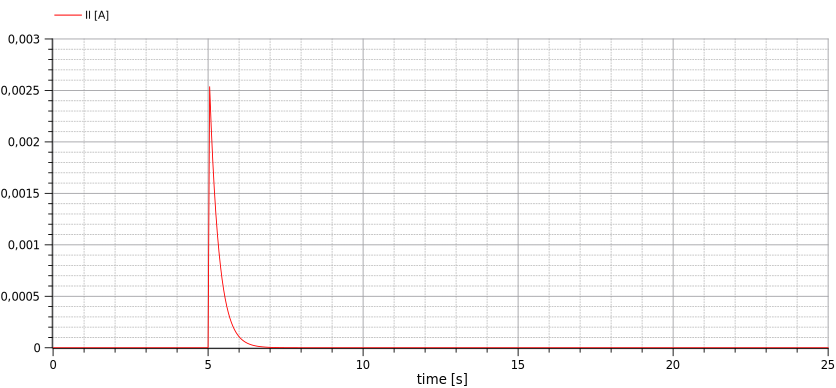
\includegraphics[width=\textwidth]{modelica/graficas/1-corrientes}
  \caption{Gráfica de Corrientes para el primer caso.}
  \label{gr:caso1:corrientes}
\end{figure}

La figura \ref{gr:caso1:tensiones} muestra el comportamiento de las tensiones
$\text{V}_s$, $\text{V}_c$, $\text{V}_r$ a lo largo del tiempo. Como es de
esperar, los cambios en las señales $\text{V}_c$ y $\text{V}_r$ varian
notablemente desde los 5 segundos hasta los 7 segundos, cuando el capacitor
está cargado. $\text{V}_s$ comienza a actuar a los 5 segundos, poniendo en
acción al circuito.

\begin{figure}[H]
  \centering
  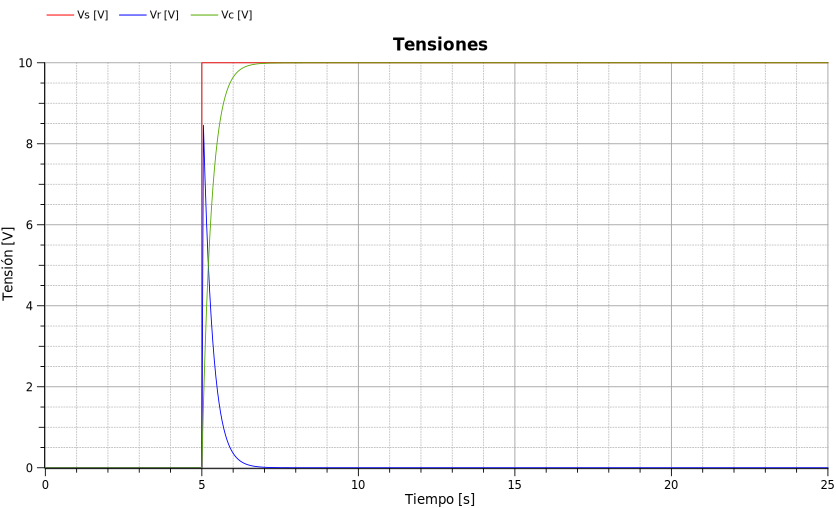
\includegraphics[width=\textwidth]{modelica/graficas/1-tensiones}
  \caption{Gráfica de Tensiones para el primer caso.}
  \label{gr:caso1:tensiones}
\end{figure}
